\PassOptionsToPackage{dvipsnames,svgnames,table}{xcolor}
\documentclass[11pt]{article}
\usepackage[a4paper,margin=22mm]{geometry}
\usepackage[no-math]{fontspec}
\setmainfont{DejaVu Serif}
\usepackage{amsmath,amssymb,amsthm,mathtools,graphicx,xcolor,hyperref,xurl,xspace,ifthen,enumerate}
\usepackage[shortlabels]{enumitem}
\setlength{\emergencystretch}{4em}
\AtBeginDocument{\special{pdf:mapline pzdr Dingbats <uzdr.pfb}}
\SetMathAlphabet{\mathbf}{normal}{OT1}{cmr}{bx}{n}
\SetMathAlphabet{\mathbf}{bold}{OT1}{cmr}{bx}{n}
\newtheorem{theo}{Theorem}[section]
\newtheorem{lemm}[theo]{Lemma}
\newtheorem{thm}[theo]{Theorem}
\newtheorem{proposition}[theo]{Proposition}
\newtheorem{corollary}[theo]{Corollary}
\newtheorem{definition}[theo]{Definition}
\newtheorem{theorem}[theo]{Theorem}
\newtheorem*{remas*}{Remarks}
\newtheorem{remas}[theo]{Remarks}
\newtheorem*{exam*}{Example}
\newtheorem{ques}[theo]{Question}
\providecommand{\og}{«\nobreakspace}
\providecommand{\fg}{\nobreakspace»}
\newtheorem{lem}[theo]{Lemma}
\newtheorem{lemma}[theo]{Lemma}
\newtheorem{prop}[theo]{Proposition}
\newtheorem{coro}[theo]{Corollary}
\newtheorem{corol}[theo]{Corollary}
\newtheorem*{conj*}{Conjecture}
\newtheorem{conj}[theo]{Conjecture}
\newtheorem{conjecture}[theo]{Conjecture}
\newtheorem{Proposition}[theo]{Proposition}
\newtheorem{theoreme}[theo]{Theorem}
\theoremstyle{definition}
\newtheorem{defi}[theo]{Definition}
\newtheorem{exam}[theo]{Example}
\newtheorem{exem}[theo]{Example}
\newtheorem{remark}[theo]{Remark}
\newtheorem{example}[theo]{Example}
\newtheorem{exams}[theo]{Examples}
\newtheorem{rema}[theo]{Remark}
\newtheorem{nota}[theo]{Notation}
\newtheorem{notation}[theo]{Notation}
\newtheorem*{notas}{Notations}
\newtheorem{result}[theo]{Result}
\newtheorem{question}[theo]{Question}
\newtheorem{prob}[theo]{Problem}
\newtheorem*{rema*}{Remark}
\newtheorem*{defi*}{Definition}
\newtheorem*{theo*}{Theorem}
\newtheorem*{lemm*}{Lemma}
\newtheorem*{prop*}{Proposition}
\newcommand{\enoncename}{}
\newtheorem{corpusenonce}[theo]{\enoncename}
\newenvironment{enonce}[2][]{\renewcommand{\enoncename}{#2}\begin{corpusenonce}}{\end{corpusenonce}}
\newenvironment{enonce*}[2][]{\par\medskip\noindent\textbf{#2.}\itshape}{\par\medskip}
\newenvironment{proofc}[1][\proofname]{\begin{proof}[#1]}{\end{proof}}
\newcommand{\Mc}{\mathcal{M}}
\newcommand{\pointir}{.\ ---\ }
\newcommand{\equalenv}[2]{\expandafter\let\csname#1\expandafter\endcsname\csname#2\endcsname\expandafter\let\csname end#1\expandafter\endcsname\csname end#2\endcsname}
\providecommand{\diagbox}[3][]{\begin{tikzpicture}[x=1em,y=1em,baseline=(current bounding box.center)]\useasboundingbox(0,0) rectangle(3,1.4);\draw(0,1.4)--(3,0);\node at(.5,.3){#2};\node at(2.5,1.1){#3};\end{tikzpicture}}
\providecommand{\eg}{e.g.\ }
\providecommand{\ie}{i.e.\ }
\providecommand{\cf}{cf.\ }
\providecommand{\longthanks}[1]{\par\smallskip\noindent #1\par\smallskip}
\providecommand{\qbinom}[2]{\genfrac{[}{]}{0pt}{}{#1}{#2}}

\providecommand{\mathof}[1]{\mathrm{#1}}

\numberwithin{equation}{section}


\def\endappendix{}


\newfontfamily\CorpusFiniteLMMath[Path=/usr/share/texmf/fonts/opentype/public/lm-math/]{latinmodern-math.otf}
\DeclareRobustCommand{\iddots}{\mathinner{\text{\CorpusFiniteLMMath\char"22F0}}}
\DeclareRobustCommand{\ddots}{\mathinner{\text{\CorpusFiniteLMMath\char"22F1}}}
\DeclareRobustCommand{\dddot}{\PackageError{corpus-finite-diagonal-dots}{Uninventoried dot control}{Only the three literal iddots and three literal ddots in the source symbolic array are approved.}}
\DeclareRobustCommand{\ddddot}{\PackageError{corpus-finite-diagonal-dots}{Uninventoried dot control}{Only the three literal iddots and three literal ddots in the source symbolic array are approved.}}

% Unused ytableau import omitted; no tableau macro occurs in retained native body.
\usepackage{xcolor}
\usepackage{tikz,tkz-euclide}

\newcommand{\x}{\mathbf{x}}
\newcommand{\la}{\lambda}
\newcommand{\y}{\mathbf{y}}
\newcommand{\A}{\mathcal{A}}

\DeclareMathOperator{\ASM}{ASM}
\DeclareMathOperator{\TSPP}{TSPP}
\DeclareMathOperator{\CSSPP}{CSSPP}
\DeclareMathOperator{\MT}{MT}
\DeclareMathOperator{\sgn}{sgn}
\DeclareMathOperator{\diag}{diag}
\DeclareMathOperator{\inv}{inv}
\DeclareMathOperator{\ct}{CT}
\DeclareMathOperator{\Id}{Id}
\DeclareMathOperator{\asym}{\mathbf{ASym}}

\newcommand{\red}[1]{{\color{red}{#1}}}
\newcommand{\blue}[1]{{\color{blue}{#1}}}
\newcommand{\cyan}[1]{{\color{cyan}{#1}}}
\newcommand{\green}[1]{{\color{green}{#1}}}

\newmuskip\pFqmuskip

\newcommand*\pFq[6][8]{
	\begingroup 
	\pFqmuskip=#1mu\relax
	\mathchardef\normalcomma=\mathcode`,
	\mathcode`\,=\string"8000
	\begingroup\lccode`\~=`\,
	\lowercase{\endgroup\let~}\pFqcomma
	{}_{#2}F_{#3}{\left[\left.\genfrac..{0pt}{}{#4}{#5}\right|#6\right]}
	\endgroup
}
\newcommand{\pFqcomma}{{\normalcomma}\mskip\pFqmuskip}

\newcommand{\PlanePartition}[1]{\PlanePartitionColour{#1}{1}}
	\newcounter{x}
	\newcounter{y}
	\newcounter{z}
	\newcounter{help}

\newcommand{\PlanePartitionColour}[2]{
	\foreach \m [count=\y] in {#1}{	
		\foreach \z [count=\x] in \m{
			\setcounter{x}{\x}		
			\ifnum \z > 0		
				\TopBoundary{\x}{-\y}{\z}{#2}	
			\fi			
			\ifnum \x > 1				
				\ifnum \z < \thez				
					\setcounter{help}{\z}
					\addtocounter{help}{1}
					\foreach \zz in {\thehelp,...,\thez}{					
						\RightBoundary{(\x -1)}{(-\y)}{\zz}{#2}	
					}											
				\fi
			\fi
			\ifnum \y > 1		
				\foreach \mm [count=\yy] in {#1}{
				\ifnum \yy = \they		
				\foreach \zz [count=\xx] in \mm{	
				\ifnum \xx = \x	
				\ifnum \zz > \z	
					\setcounter{help}{\zz}
					\addtocounter{help}{-1}	
					\foreach \zzz in {\z,...,\thehelp}{
						\LeftBoundary{(\x -1)}{(1-\yy)}{\zzz}{#2}	
					}
				\fi
				\fi
				}
				\fi
				}
			\fi		
			\setcounter{z}{\z}
		}						
		\ifnum \thez >0	
			\foreach \z in {1,...,\thez}{
				\RightBoundary{\thex}{-\y}{\z}{#2}	
			}
		\fi
		\setcounter{y}{\y}
	}							
	\foreach \mm [count=\yy] in {#1}{	
	\ifnum \yy = \they
	\foreach \zz [count=\xx] in \mm{
	\ifnum \zz >0
		\foreach \zzz in {1,...,\zz}{
			\LeftBoundary{(\xx -1)}{(1-\yy)}{(\zzz-1)}{#2}
		}
	\fi
	}
	\fi
	}
	
}

\newcommand{\RightBoundaryColour}[4]{
\begin{scope}[xshift= 1cm*cos(30)*(#1+#2) , yshift=1cm*#3+1cm*sin(30)*(#2-#1)]
\draw [fill=#4] (0,0) -- ({1*cos(30)},{1*sin(30)}) -- ({1*cos(30)},{-1*sin(30)}) -- (0,-1) -- (0,0);
\end{scope}
}
\newcommand{\LeftBoundaryColour}[4]{
\begin{scope}[xshift= 1cm*cos(30)*(#1+#2) , yshift=1cm*#3+1cm*sin(30)*(#2-#1)]
\draw (0,0)[fill=#4] -- ({-1*cos(30)},{1*sin(30)}) -- ({-1*cos(30)},{-1*sin(30)}) -- (0,-1) -- (0,0);
\end{scope}
}
\newcommand{\TopBoundaryColour}[4]{
\begin{scope}[xshift= 1cm*cos(30)*(#1+#2) , yshift=1cm*#3+1cm*sin(30)*(#2-#1)]
\draw (0,0)[fill=#4] -- ({1*cos(30)},{1*sin(30)}) -- (0,1) -- ({-1*cos(30)},{1*sin(30)}) -- (0,0);
\end{scope}
}

\newcommand{\RightBoundary}[4]{
\ifnum #4 =1
	\RightBoundaryColour{#1}{#2}{#3}{green!80!black}
\else \ifnum #4=2
	\RightBoundaryColour{#1}{#2}{#3}{darkgray}
\else
	\RightBoundaryColour{#1}{#2}{#3}{white}
	\fi
\fi
}
\newcommand{\LeftBoundary}[4]{
\ifnum #4 =1
	\LeftBoundaryColour{#1}{#2}{#3}{blue}
\else \ifnum #4 = 2
	\LeftBoundaryColour{#1}{#2}{#3}{lightgray}
\else
	\LeftBoundaryColour{#1}{#2}{#3}{white}
	\fi
\fi
}
\newcommand{\TopBoundary}[4]{
\ifnum #4 =1
	\TopBoundaryColour{#1}{#2}{#3}{red}
\else \ifnum #4=2
	\TopBoundaryColour{#1}{#2}{#3}{white}
\else
	\TopBoundaryColour{#1}{#2}{#3}{white}
	\fi
\fi
}

\newcommand{\PlanePartitionWhite}[1]{\PlanePartitionColour{#1}{3}}

\newcommand{\Square}[2]{\draw[xshift=#1 cm,yshift=#2 cm] (0,0) -- (0,1) -- (1,1) -- (1,0) -- (0,0);}

\newcommand{\VertexLU}[2]{
\vertcross{#1}{#2}
\LtriangleL{#1}{#2}
\LtriangleR{#1}{#2}
\UtriangleU{#1}{#2}
\UtriangleD{#1}{#2}
}
\newcommand{\VertexLD}[2]{
\vertcross{#1}{#2}
\LtriangleL{#1}{#2}
\LtriangleR{#1}{#2}
\DtriangleU{#1}{#2}
\DtriangleD{#1}{#2}
}
\newcommand{\VertexRU}[2]{
\vertcross{#1}{#2}
\RtriangleL{#1}{#2}
\RtriangleR{#1}{#2}
\UtriangleU{#1}{#2}
\UtriangleD{#1}{#2}
}
\newcommand{\VertexRD}[2]{
\vertcross{#1}{#2}
\RtriangleL{#1}{#2}
\RtriangleR{#1}{#2}
\DtriangleU{#1}{#2}
\DtriangleD{#1}{#2}
}
\newcommand{\VertexOne}[3][black]{
\vertcross{#2}{#3}
\begin{scope}[#1]
\RtriangleL{#2}{#3}
\LtriangleR{#2}{#3}
\UtriangleU{#2}{#3}
\DtriangleD{#2}{#3}
\end{scope}
}
\newcommand{\VertexMinus}[3][black]{
\vertcross{#2}{#3}
\begin{scope}[#1]
\LtriangleL{#2}{#3}
\RtriangleR{#2}{#3}
\DtriangleU{#2}{#3}
\UtriangleD{#2}{#3}
\end{scope}
}

\newcommand{\vertcross}[2]{
\draw[xshift=#1 cm,yshift=#2 cm] (-.85,0) -- (.85,0);
\draw[xshift=#1 cm,yshift=#2 cm] (0,-.85) -- (0,.85);
\draw[fill] (#1,#2) circle [radius=0.07];
}

\newcommand{\RtriangleR}[2]{
\draw[fill, draw=none, xshift=#1 cm,yshift=#2 cm] (.4,.1) -- (.4,-.1) -- (.6,0);
}
\newcommand{\RtriangleL}[2]{
\draw[fill, draw=none, xshift=#1 cm,yshift=#2 cm] (-.6,.1) -- (-.6,-.1) -- (-.4,0);
}
\newcommand{\LtriangleR}[2]{
\draw[fill, draw=none, xshift=#1 cm,yshift=#2 cm] (.6,.1) -- (.6,-.1) -- (.4,0);
}
\newcommand{\LtriangleL}[2]{
\draw[fill, draw=none, xshift=#1 cm,yshift=#2 cm] (-.4,.1) -- (-.4,-.1) -- (-.6,0);
}
\newcommand{\UtriangleU}[2]{
\draw[fill, draw=none, xshift=#1 cm,yshift=#2 cm] (-.1,.4) -- (.1,.4) -- (0,.6);
}
\newcommand{\UtriangleD}[2]{
\draw[fill, draw=none, xshift=#1 cm,yshift=#2 cm] (-.1,-.6) -- (.1,-.6) -- (0,-.4);
}
\newcommand{\DtriangleU}[2]{
\draw[fill, draw=none, xshift=#1 cm,yshift=#2 cm] (-.1,.6) -- (.1,.6) -- (0,.4);
}
\newcommand{\DtriangleD}[2]{
\draw[fill, draw=none, xshift=#1 cm,yshift=#2 cm] (-.1,-.4) -- (.1,-.4) -- (0,-.6);
}
















  



\begin{document}
\section*{\raggedright 995: Multivariate weighted alternating-sign matrices have a totally-symmetric-plane-partition Schur expansion}
\noindent\textbf{Author:} Fischer, Ilse; Schreier-Aigner, Florian\par\noindent\textbf{Source:} Alternating sign matrices and totally symmetric plane partitions. Algebraic Combinatorics 7 (2024), publisher version, DOI 10.5802/alco.374. \url{https://alco.centre-mersenne.org/articles/10.5802/alco.374/}
\par\noindent\textbf{License:} CC BY 4.0, \url{https://creativecommons.org/licenses/by/4.0/}. The original publisher PDF cover has the explicit license notice. See the saved source/license records.
\par\noindent\textbf{Editorial material note (not author text):} Finite typography note: the exact three upward and three downward diagonal-ellipsis controls in native623--632 use only pinned installed LatinModernMath U+22F0/U+22F1 as mathinner. Orientations preserve the original categories; dot stroke/size/spacing and vertical placement may differ. Every symbolic array entry and native position remains intact, with all six actual output uses and neighboring formulas checked. No unavailable package is acquired or emulated. The selected problem is original Theorem1.1 only: the exact uniform multivariate weighted-ASM generating function equals the TSPP Schur expansion. Complete author Sections1--5 retain all TSPP/refined determinant, ASM/six-vertex/monotone-triangle definitions, the full independent algebraic antisymmetrizer-to-determinant Lemma4.1 proof and complete coefficient extraction/Durfee deletion recursion through989. The subsequent CSSPP specialization theorem and optional alternative combinatorial proof in AppendixA are unselected; only their original printed references remain. The independent full algebraic route proves the selected unit without those omitted alternatives. Every original TikZ illustration, caption and mathematical formula is editable author TeX. All proof text and formulas below are editable author TeX. Mathematical wording, language and proof order are retained. Only the article class, title matter and bibliography presentation are adapted for independent compilation; no proof has been generated or repaired.
\par\noindent\textbf{Editorial difficulty:} H3: The proof derives an antisymmetrizer-to-determinant identity, extracts Schur coefficients, and matches a Durfee-square deletion recursion with the refined plane-partition determinant. This nonroutine uniform multivariate identity is preserved with the full recurrence proof, not merely ordinary ASM enumeration.
\medskip\hrule\medskip
\noindent\textbf{Author statement, complete proof and local supporting text follow in source order.}
\section{Introduction}
\emph{Plane partitions} were first studied by MacMahon~\cite{MacMahon97} at the end of the 19th century, however found broader interest in the combinatorial community starting in the second half of the last century. \emph{Alternating sign matrices} (ASMs) on the other hand were introduced by Robbins and Rumsey~\cite{RobbinsRumsey86} in the early 1980s. Together with Mills~\cite{MillsRobbinsRumsey82}, they conjectured that the number of $n \times n$ ASMs is given by $\prod_{i=0}^{n-1} \frac{(3i+1)!}{(n+i)!}$. Stanley then pointed out that these numbers had appeared before in the work of Andrews~\cite{Andrews79} as the enumeration formula for a certain class of plane partitions, called \emph{descending plane partitions} (DPPs). Soon after that Mills, Robbins and Rumsey~\cite{MillsRobbinsRumsey86} observed (conjecturally) that this formula also counts another class of plane partitions, namely \emph{totally symmetric self-complementary plane partitions} (TSSCPPs). Although these conjectures have all been proved since then, see among others~\cite{Andrews94,Zeilberger96}, it is mostly agreed that there is no good combinatorial understanding of this relation between ASMs and certain classes of plane partitions since we lack transparent combinatorial proofs of these results. However, Konvalinka and the first author~\cite{cube,FischerKonvalinka20plus} have recently established complicated bijective proofs (involving a generalisation of the involution principle) for two non-trivial alternating sign matrix result. On the one hand, they have provided a bijective proof for the fact that $n \times n$ ASMs are counted by the product formula given above and, on the other hand, they have constructed a bijective proof for 
an identity that implies the equinumerosity of ASMs and DPPs.

One purpose of this paper is to relate ASMs to yet another class of plane partitions, namely \emph{totally symmetric plane partitions} (TSPPs), in a new way. This relation is via a certain Schur polynomial expansion. 
Other known relations between ASMs and TSPPs are the fact that the number of symmetric plane partitions inside an \mbox{$(n,n,n-1)$}-box is the product of the number of TSPPs inside an $(n-1,n-1,n-1)$-box and the number of ASMs of size $n$, see~\cite{Fischer05}, and via posets, see \cite[Section 8]{Striker11}.

The following symmetric functions are studied in this paper
\[
\A_{n,k}(r,u,v,w; \x) := \sum_{T \in \TSPP_{n-1}} \omega(T) s_{\pi_k(T)}(\x),
\]
where $s_{\pi_k(T)}(\x)$ are Schur functions,
the sum is over totally symmetric plane partitions inside an $(n-1,n-1,n-1)$-box, $\pi_k(T)$ is a slight modification of the diagonal of $T$ and $\omega(T)$ is a monomial in $r,u,v,w$ that depends on the parameters in the Frobenius notation of $\pi_0(T)$.
All notations in the introduction are defined in the following sections. For $n=3$, the function $\A_{3,k}(r,u,v,w,\x)$ is a sum over all TSPPs inside a $(2,2,2)$-box, see Figure~\ref{fig: Example for Ank}, and it is equal to
\[
v^3 + r  u v^2 s_{(1^{k+1})}(\x) + r  uv w s_{(1^{k+2})}(\x) + r  u^2 v  s_{(2,1^{k+1})}(\x) + r^2u^3 s_{(2^{k+2})}(\x).
\]

\begin{figure}
\begin{center}
	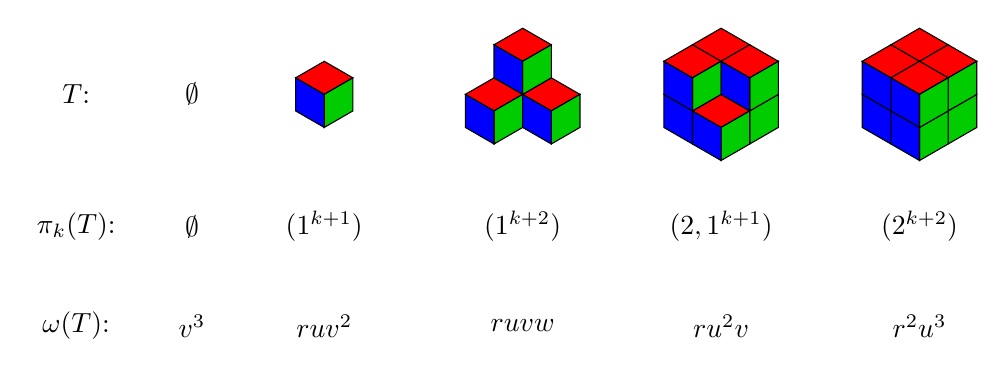
\begin{tikzpicture}
	\begin{scope}[scale=0.42]
		\node at (-1.5,0) {$T$:};
		\node at (2,0) {$\emptyset$};
		\begin{scope}[xshift=6cm]
			\PlanePartition{{1,0},{0,0}}
		\end{scope}
		\begin{scope}[xshift=12cm]
			\PlanePartition{{2,1},{1,0}}
		\end{scope}
		\begin{scope}[xshift=18cm]
			\PlanePartition{{2,2},{2,1}}
		\end{scope}
		\begin{scope}[xshift=24cm]
			\PlanePartition{{2,2},{2,2}}
		\end{scope}
	\end{scope}
	\begin{scope}[scale=0.42, yshift=-6cm,]
		\node at (-1.5,2) {$\pi_k(T)$:};
		\node at (2,2) {$\emptyset$};
		\node at (6,2) {$(1^{k+1})$};
		\node at (12,2) {$(1^{k+2})$};
		\node at (18,2) {$(2,1^{k+1})$};
		\node at (24,2) {$(2^{k+2})$};
	\end{scope}
	\begin{scope}[scale=0.42, yshift=-7cm]
		\node at (-1.5,0) {$\omega(T)$:};
		\node at (2,0) {$ v^3$};
		\node at (6,0) {$r  u v^2$};
		\node at (12,0) {$r  u v w$};
		\node at (18,0) {$r  u^2 v$};
		\node at (24,0) {$r^2 u^3$};
	\end{scope}
	\end{tikzpicture}
\end{center}
\caption{\label{fig: Example for Ank} Totally symmetric plane partitions inside a $(2,2,2)$-box, their associated weight $\omega(T)$ and the partitions $\pi_k(T)$.}
\end{figure}

Our first main result states that in the special case $k=1$, the above functions give the Schur polynomial expansion of a weighted generating function for ASMs, which has recently been introduced by the authors in~\cite{FischerSchreierAigner23}.

\begin{thm}
\label{thm: main thm 1}
For all positive integers $n$, the weighted generating function for ASMs with respect to the weight $\omega_A$ is equal to
\begin{equation}
\label{eq: main thm 1}
\sum_{A \in \ASM_n} \omega_A(u,v,w;\x) = \A_{n,1}(1, u,v,w;\x).
\end{equation}
\end{thm}
The relevant definitions for this theorem can be found in Section~\ref{sec: ASM gen fct}. In particular, $\omega_A(u,v,w;\x)$ is defined in 
\eqref{def:omega}.

Our proof of this result is (mostly) non-combinatorially, and thus it adds another problem to the growing zoo of (obviously challenging) bijective proof problems related to ASMs and plane partitions. More specifically, it suggests that there is a bijection between the down-arrowed monotone triangles\footnote{These are certain decorated monotone triangles. Monotone triangles are in easy bijective correspondence with ASMs.} from~\cite{FischerSchreierAigner23}, and pairs of totally symmetric plane partitions and semistandard Young tableaux. Moreover,~\eqref{eq: main thm 1} involves $n+3$ parameters, and, therefore, we have a considerable number of equidistributed statistics that could help in finding such a bijection. These $n+3$ statistics are the exponents of $u,v,w,x_1,\ldots,x_n$, and
it is interesting to note that, on the alternating sign matrix side, 
the exponent of $x_i$ is closely related to the difference of the $i$-th and $(i-1)$-st row sum of the monotone triangles, while the exponent of $x_i$ on the plane partition side is precisely the  difference of the $i$-th and $(i-1)$-st row sum in the Gelfand--Tsetlin pattern when interpreting the Schur polynomial as the generating function of Gelfand--Tsetlin patterns.

In the second part of our paper, we consider the case of general $k$ and connect the family $\A_{n,k}$ of symmetric functions to another family of plane partitions, namely \emph{column strict shifted plane partitions} (CSSPPs) of class $k$. CSSPPs of class~$k$ form a family of plane partitions, generalising cyclically symmetric plane partitions (CSPPs) and DPPs in the sense that they are in bijection to CSPPs for $k=0$ and to DPPs for~$k=2$. 
Let $\CSSPP_{n,k}(r,t)$ denote a certain generating function of CSSPPs of class~$k$ with at most $n$ entries in the first row; for the definitions see Section~6. Then our second main theorem states the following.

\begin{thm}
\label{thm: main thm 2}
Let $n$ be a positive integer and let $\mathbf{1}=(1, \ldots, 1)$. Then,
\begin{align}
\label{eq: Ank CSSPP 1}
\A_{n+1,0}(r,1,1,t;\mathbf{1})&=\CSSPP_{n,0}(r,t+2),\\
\label{eq: Ank CSSPP 2}
\A_{n+1,k}(r,1,1,-1;\mathbf{1})&=\CSSPP_{n,2k}(r,1),\\
\label{eq: Ank CSSPP 3}
\A_{n+1,k}(r,1,1,0;\mathbf{1})&=\CSSPP_{n,k}(r,2).
\end{align}
\end{thm}
For $k=1$, the identity~\eqref{eq: Ank CSSPP 2} is closely related a special case of \cite[Theorem 2.6]{FischerSchreierAigner23}. The choice of the parameters $(u,v,w)=(1,1,-1)$ in 
\eqref{eq: Ank CSSPP 2} corresponds to the straight enumeration of ASMs, while the choice $(u,v,w)=(1,1,0)$ in 
\eqref{eq: Ank CSSPP 3} corresponds to the $2$-enumeration of ASMs, which is related to the straight enumeration of the Aztec diamond.

The structure of the paper is as follows. In Section~\ref{sec: TSPPs}, we  recall some basics of plane partitions and introduce the family $\A_{n,k}$ of symmetric functions in detail. In Section~\ref{sec: ASM gen fct}, we provide the definition of the symmetric generating function for ASMs and relate the weight for ASMs to the six-vertex model. Section~\ref{sec: antisym to det} contains Lemma ~\ref{lem: general}, which allows us to express certain antisymmetrizer as determinants. We provide two proofs of this lemma: one is very short and uses linear algebra. The second is complicated and combinatorial in nature and based on directed graphs. The latter can be found in the appendix. While this combinatorial proof does not seem to be insightful at first glance, its complexity might serve as an explanation why it is so hard to come up with bijective proofs in this field, see~\cite{cube} for more discussion of this point. Section~\ref{sec: proof of mt 1} contains the proof of Theorem~\ref{thm: main thm 1}. In Section~6, we recall CSSPPs and provide in Lemma~6.2 a determinantal description of $\A_{n,k}$ closely related to the Giambelli identity for Schur functions. The proof of Theorem~\ref{thm: main thm 2} is presented in Section~7.

An extended abstract containing parts of Section~\ref{sec: TSPPs}--\ref{sec: proof of mt 1} was published in the proceedings of FPSAC 2020~\cite{AignerFischerKonvalinkaNadeauTewari20}.

\section{A family of symmetric functions related to TSPPs}
\label{sec: TSPPs}

A \emph{partition} $\la=(\la_1,\ldots,\la_n)$ is a weakly decreasing sequence of non-negative integers (we deviate from the more usual definition where parts have to be positive). We identify a partition $\la$ with its \emph{Young diagram}, which is a collection of left-justified boxes with $\la_i$ boxes in the $i$-th row from the bottom (using French notation). The \emph{conjugate} $\la^\prime$ of $\la$ is the partition obtained by reflecting the Young diagram along the $y=x$ axis, i.e., $\la^\prime_i=|\{j: \la_j \geq i\}|$. The \emph{Durfee square} of a partition $\la$ is the largest square which fits into the Young diagram. The \emph{Frobenius notation} of a partition $\la$ is $(\la_1-1,\ldots,\la_l-l|\la_1^\prime-1,\ldots,\la_l^\prime-l)$, where $l= \max_i\{ \la_i \geq i \}$ is the length of the Durfee square of $\la$.
 
Let $k$ be a non-negative integer. A \emph{$k$-tall partition}\footnote{For $k=0$, these objects were defined in \cite[Ex 6.16(bb), p.223]{Stanley99} without a name, and for $k=1$ in~\cite{AignerFischerKonvalinkaNadeauTewari20} as modified balanced partitions.} $\la$ of size $n$ is a partition $\la=(\la_1,\ldots,\la_{n+k-1})$ with $\la_1\leq n-1$ that satisfies $\la_i +k \leq \la_i^\prime$ whenever $\la_i \geq i$. See Figure~\ref{fig: mod bal part n=3} for an example.
 If $\la$ has Frobenius notation $(a_1,\ldots,a_l|b_1+k,\ldots,b_l+k)$, then $\la$ is a $k$-tall partition iff $a_i \leq b_i$ for all $1 \leq i \leq l$. Let $N$ denote a unit north-step and $E$ a unit east-step. The map
\begin{multline*}
(a_1,\ldots,a_l|b_1+k,\ldots,b_l+k) \mapsto \\
N^{b_l+1}E^{a_l+1}N^{b_{l-1}-b_l}E^{a_{l-1}-a_l} \cdots N^{b_1-b_2}E^{a_1-a_2}N^{n-b_1-1}E^{n-a_1-1}
\end{multline*}
and $(|) \mapsto N^nE^n$ is a bijection from $k$-tall partitions of size $n$ to Dyck paths of length~$2n$.

\begin{figure}
\begin{center}
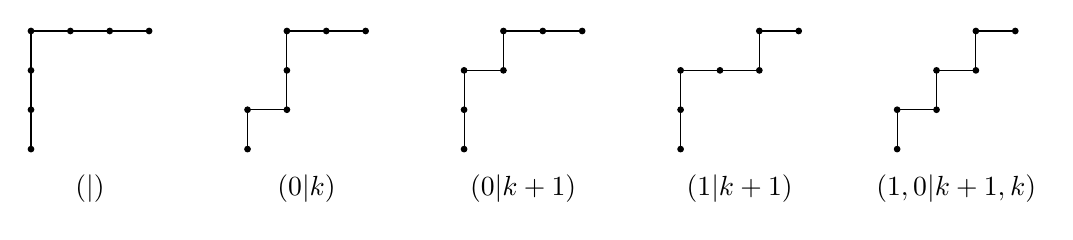
\begin{tikzpicture}
	\draw (0,0)--(0,1.5) -- (1.5,1.5);
	\draw[fill] (0,0) circle (1pt);
	\draw[fill] (0,0.5) circle (1pt);
	\draw[fill] (0,1) circle (1pt);
	\draw[fill] (0,1.5) circle (1pt);
	\draw[fill] (0.5,1.5) circle (1pt);
	\draw[fill] (1,1.5) circle (1pt);
	\draw[fill] (1.5,1.5) circle (1pt);
	\node at (.75,-.5) {$(|)$};
\begin{scope}[xshift=2.75cm]
	\draw (0,0)--(0,.5) -- (.5,.5) -- (0.5,1.5) -- (1.5,1.5);
	\draw[fill] (0,0) circle (1pt);
	\draw[fill] (0,0.5) circle (1pt);
	\draw[fill] (0.5,.5) circle (1pt);
	\draw[fill] (0.5,1) circle (1pt);
	\draw[fill] (0.5,1.5) circle (1pt);
	\draw[fill] (1,1.5) circle (1pt);
	\draw[fill] (1.5,1.5) circle (1pt);
	\node at (.75,-.5) {$(0|k)$};	
\end{scope}
\begin{scope}[xshift=5.5cm]
	\draw (0,0)--(0,1) -- (0.5,1) -- (0.5,1.5) -- (1.5,1.5);
	\draw[fill] (0,0) circle (1pt);
	\draw[fill] (0,0.5) circle (1pt);
	\draw[fill] (0,1) circle (1pt);
	\draw[fill] (0.5,1) circle (1pt);
	\draw[fill] (0.5,1.5) circle (1pt);
	\draw[fill] (1,1.5) circle (1pt);
	\draw[fill] (1.5,1.5) circle (1pt);
	\node at (.75,-.5) {$(0|k+1)$};
\end{scope}
\begin{scope}[xshift=8.25cm]
	\draw (0,0)--(0,1) -- (1,1) -- (1,1.5) -- (1.5,1.5);
	\draw[fill] (0,0) circle (1pt);
	\draw[fill] (0,0.5) circle (1pt);
	\draw[fill] (0,1) circle (1pt);
	\draw[fill] (0.5,1) circle (1pt);
	\draw[fill] (1,1) circle (1pt);
	\draw[fill] (1,1.5) circle (1pt);
	\draw[fill] (1.5,1.5) circle (1pt);
	\node at (.75,-.5) {$(1|k+1)$};
\end{scope}
\begin{scope}[xshift=11cm]
	\draw (0,0)--(0,.5) -- (.5,.5) -- (.5,1) -- (1,1) -- (1,1.5) -- (1.5,1.5);
	\draw[fill] (0,0) circle (1pt);
	\draw[fill] (0,0.5) circle (1pt);
	\draw[fill] (.5,.5) circle (1pt);
	\draw[fill] (0.5,1) circle (1pt);
	\draw[fill] (1,1) circle (1pt);
	\draw[fill] (1,1.5) circle (1pt);
	\draw[fill] (1.5,1.5) circle (1pt);
	\node at (.75,-.5) {$(1,0|k+1,k)$};
\end{scope}
\end{tikzpicture}
\caption{\label{fig: mod bal part n=3} All $k$-tall partitions of size $3$ in Frobenius notation together with their associated Dyck paths.}
\end{center}
\end{figure}
 
A \emph{plane partition} $\pi$ inside an $(a,b,c)$-box is an array $(\pi_{i,j})_{1 \leq i \leq a, 1 \leq j \leq b}$ of non-negative integers less than or equal to $c$, with weakly decreasing rows and columns, i.e., $\pi_{i,j} \geq \pi_{i,j+1}$ and  $\pi_{i,j} \geq \pi_{i+1,j}$. We can visualise a plane partition $\pi$ as stacks of unit cubes by putting $\pi_{i,j}$ cubes at position $(i,j)$, see Figure~\ref{fig: ex PP}. The visualisation allows an equivalent definition of plane partitions as follows. A plane partition $\pi$ inside an $(a,b,c)$-box is a subset of $[a]\times[b] \times[c]$, where $[n]=\{1,\ldots,n\}$, such that $(i,j,k) \in \pi$ implies $(i^\prime,j^\prime,k^\prime) \in \pi$ for all $i^\prime \leq i, j^\prime \leq j, k^\prime \leq k$.
\begin{figure}
\begin{center}
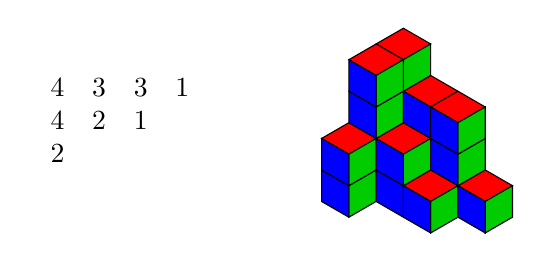
\begin{tikzpicture}
\begin{scope}
	\node at (0,0) {$\begin{array}{cccc}
	4 & 3 & 3 & 1\\
	4 & 2 & 1 \\
	2
	\end{array}$};
	\end{scope}
	\begin{scope}[scale=0.4, xshift=9cm, yshift=-1cm]
		\PlanePartition{{4,3,3,1},{4,2,1,0},{2,0,0,0}}
	\end{scope}
\end{tikzpicture}
\caption{\label{fig: ex PP} A plane partition inside a $(3,4,4)$-box, with $0$ entries omitted, and its graphical representation as stacks of cubes.}
\end{center}
\end{figure}
A plane partition is called \emph{totally symmetric} if for every $(i,j,k) \in \pi$, all permutations of $(i,j,k)$ are also elements of $\pi$. We denote by $\TSPP_n$ the set of totally symmetric plane partitions (TSPPs) inside an $(n,n,n)$-box. Let $T=(T_{i,j})_{1\leq i,j \leq n}$ be a totally symmetric plane partition, $\diag(T)=(T_{i,i})_{1 \leq i \leq n}^\prime$ its diagonal (note that we conjugate) and $(a_1,\ldots,a_l|b_1,\ldots,b_l)$ the Frobenius notation of $\diag(T)$. The partition $\diag(T)$ describes the shape which is obtained by intersecting the visualisation of $T$ as stacks of cubes with the $x=y$ plane. See Figure~\ref{fig:LGV} right for an example. We associate with $T$ the partition $\pi_k(T)=(a_1,\ldots,a_l|b_1+k,\ldots,b_l+k)$ of size $n+1$. As a consequence of the next proposition, we obtain that $\pi_k(T)$ is a $k$-tall partition of size $n+1$.

\begin{prop}
\label{prop: TSSPP refinement}
Let $\lambda=(a_1,\ldots,a_l|b_1+k,\ldots,b_l+k)$ be a $k$-tall partition. The number of totally symmetric plane partitions $T$ with $\pi_k(T)=\lambda$ is given by
\[
\det_{1 \leq i,j \leq l}\left( \binom{b_i}{a_j}\right).
\]
\end{prop}
\begin{proof}
This is a classical application of the Lindstr\"om--Gessel--Viennot theorem~\cite{GesselViennot85,Lindstroem73}, see also~\cite{Stembridge95}. 
We sketch the proof on the example in Figure~\ref{fig:LGV}.  

TSPPs of order $n$ clearly correspond to lozenge tilings of a regular hexagon with side lengths $n$ that are symmetric with respect to the vertical symmetry axis as well as rotation of $120^\circ$. By this symmetry, it suffices to know a sixth of the lozenge tiling. In our example, we choose the sixth that is in the wedge of the red dotted rays.
\begin{figure}
\centering
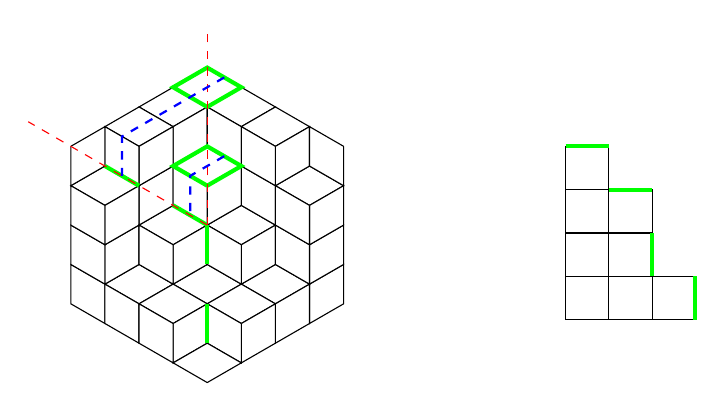
\begin{tikzpicture}
\begin{scope}[scale=0.5]
\PlanePartitionWhite{{4,4,4,3},{4,3,2,1},{4,2,1,1},{3,1,1,0}}
\RightBoundary{0}{-4}{4}{3}
\LeftBoundary{4}{0}{4}{3}
\TopBoundary{4}{-4}{0}{3}
\draw [color=green, line width=1.5pt] (0,1) -- ({1*cos(30)},{1+1*sin(30)}) -- (0,2) -- ({-1*cos(30)},{1+1*sin(30)}) -- (0,1);
\draw [color=green, line width=1.5pt] (0,3) -- ({1*cos(30)},{3+1*sin(30)}) -- (0,4) -- ({-1*cos(30)},{3+1*sin(30)}) -- (0,3);
\draw [color=green, line width=1.5pt] (0,-1) -- (0,0);
\draw [color=green, line width=1.5pt] (0,-3) -- (0,-2);
\draw [color=green, line width=1.5pt] (0,0) -- ({-1*cos(30)},{1*sin(30)});
\draw [color=green, line width=1.5pt] ({-3*cos(30)},{3*sin(30)}) -- ({-2*cos(30)},{2*sin(30)});
\draw [dashed, red] (0,0) -- (0,5);
\draw [dashed, red] (0,0) -- ({-5.25*cos(30)},{5.25*sin(30)});
\draw [dashed, blue, thick] ({1/2*cos(30)},{1+3/2*sin(30)}) -- ({-1/2*cos(30)},{1+1/2*sin(30)})  -- ({-1/2*cos(30)},{1/2*sin(30)});
\draw [dashed, blue, thick] ({1/2*cos(30)},{1+11/2*sin(30)}) -- ({-5/2*cos(30)},{1+5/2*sin(30)}) -- ({-5/2*cos(30)},{5/2*sin(30)});

\begin{scope}[xshift=8cm, yshift=-3.5cm, scale=1.1]
\Square{1}{4}
\Square{1}{3}
\Square{1}{2}
\Square{1}{1}
\Square{2}{3}
\Square{2}{2}
\Square{2}{1}
\Square{3}{1}
\draw [color=green, line width=1.5pt] (1,5) -- (2,5);
\draw [color=green, line width=1.5pt] (2,4) -- (3,4);
\draw [color=green, line width=1.5pt] (3,3) -- (3,2);
\draw [color=green, line width=1.5pt] (4,2) -- (4,1);
\end{scope}
\end{scope}
\end{tikzpicture}
\caption{\label{fig:LGV} Running example in the proof of Proposition~\ref{prop: TSSPP refinement} (left) and its diagonal $\diag(T)$ (right), with the corresponding edges also coloured in green.}
\end{figure} 

\noindent
Now observe that the positions of the horizontal lozenges in the upper half of the vertical symmetry axis are prescribed by the $b_i$'s, while the positions of the vertical segments in the lower part of the vertical symmetry axis are prescribed by the $a_i$'s. Both are indicated in green in Figure~\ref{fig:LGV}. By the cyclic symmetry, these green segments have corresponding segments on the red dotted ray that is not contained on the vertical symmetry axis, again indicated in green in the figure. Now the lozenge tiling is determined by the family of non-intersecting lattice paths that connect these segments with the horizontal lozenges in the upper half of the vertical symmetry axis, indicated in blue in the figure.
\end{proof}

Let $\lambda=(\lambda_1,\ldots,\lambda_n)  \subseteq (n^n)$ be a partition with Frobenius notation $(a_1,\ldots,a_l | \allowbreak b_1,\ldots,b_l)$ and define $\lambda^c=(\lambda_i^c)_{1 \leq i \leq n}$ by $\lambda_{n+1-i}^c=n-\lambda_i$. Then $\lambda^c$ is the complement of $\lambda$ inside the partition $(n^n)$ in the sense that we can fill a square of side length $n$ by the Young diagrams of $\la$ and $\lambda^c$ without overlap, see Figure~\ref{fig: ex complement of partition} for an example.
\begin{figure}
\begin{center}
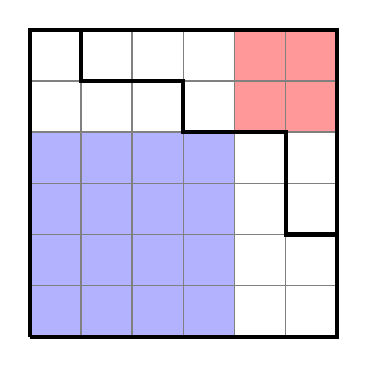
\begin{tikzpicture}
\begin{scope}[scale=.65]
\draw[fill = blue!30!white] (0,0) rectangle (4,4);
\draw[fill = red!40!white] (4,4) rectangle (6,6);
\foreach \x in {0,1,...,6}{
	\draw[gray, line width = 0.5pt] (0,\x) -- (6,\x);
	\draw[gray, line width = 0.5pt] (\x,0) -- (\x,6);
}
\draw[line width = 1.5pt] (0,0) -- (6,0) -- (6,2) -- (5,2) -- (5,4) -- (3,4) -- (3,5) -- (1,5) -- (1,6) -- (0,6)  -- (0,0);
\draw[line width = 1.5pt] (1,6) -- (6,6) -- (6,2);
\end{scope}
\end{tikzpicture}
\caption{\label{fig: ex complement of partition} The partition $\lambda=(6,6,5,5,3,1)$ in the bottom left and its complement $\lambda^c = (5,3,1,1)$ in the top right. Their corresponding Durfee squares are coloured in blue or red respectively.}
\end{center}
\end{figure}
  Let $( a_1^c,\ldots,a_L^c|b_1^c,\ldots,b_L^c)$ be the Frobenius notation of $\lambda^c$. Every box of the $x=y$ diagonal of the $n \times n$ square is either in the Durfee square of $\lambda$ or of $ \lambda^c$. Hence we have $l+L=n$. Using induction on $n$, one can show the equality of the following sets.
\begin{equation}
\label{eq: Frobenius coef of complement}
\{a_1,\ldots,a_l, b_1^c,\ldots, b_L^c \}=\{ a_1^c,\ldots,a_L^c,b_1,\ldots,b_l\}=\{0,\ldots,n-1\}
\end{equation}
For a totally symmetric plane partition $T=(T_{i,j})_{1 \leq i,j \leq n}$ inside an $(n,n,n)$-box denote by $T^c$ the complement of $T$, defined by
\[
T^c = (n-T_{n+1-i,n+1-j})_{1 \leq i,j \leq n}.
\]
The map $T \mapsto T^c$ is an involution on  totally symmetric plane partitions inside an $(n,n,n)$-box which satisfies $\pi_0(T^c) = \pi_0(T)^c$. Together with Proposition~\ref{prop: TSSPP refinement}, this implies
\begin{equation}
\label{eq: det of complement}
\det_{1 \leq i,j \leq l}\left( \binom{b_i}{a_j}\right) =
\det_{1 \leq i,j \leq n-l}\left( \binom{b_i^c}{a_j^c}\right).
\end{equation} 

Denote by $\A_{n,k}(r, u,v,w;\x)$ the symmetric polynomials in $\x=(x_1,\ldots,x_{n+k-1})$ defined by
\begin{equation}
\label{eq: def of A}
\A_{n,k}(r, u,v,w;\x)=\sum_{T \in \TSPP_{n-1}}\omega(T) s_{\pi_k(T)}(\x),
\end{equation}
where 
\begin{equation} 
\label{eq: weightpp} 
\omega(T)=r^l u^{\sum\limits_{i=1}^l (a_i+1)}  v^{\binom{n}{2}-\sum\limits_{i=1}^l (b_i+1)} w^{\sum\limits_{i=1}^l (b_i-a_i)},
\end{equation} 
if $\diag(T)$ has Frobenius notation $(a_1,\ldots,a_l|b_1,\ldots,b_l)$. We list this family of symmetric functions for $n\leq 4$.
\begin{align*}
\A_{1,k} (r, u,v,w,t;\x) &=1, \\
\A_{2,k} (r, u,v,w,t;\x) &= v + r u \,s_{(0|k)}(\x), \\
\A_{3,k} (r, u,v,w,t;\x) &=  v^3 + r  u v^2  \, s_{(0|k)}(\x) + 
	r  u v w  \,s_{(0|k+1)}(\x)+ r   u^2 v \,s_{(1|1+k)}(\x) \\
	& \quad +r^2 u^3 \,s_{(1,0|1+k,k)}(\x), \\ 
\A_{4,k} (r, u,v,w,t;\x) &=   v^6
	+r  u v^5  \,s_{(0|k)}(\x)
	+r  u v^4 w \,s_{(0|k+1)}(\x)
	+r  u^2 v^4 \,s_{(1|k+1)}(\x) \\
	& \quad 	+r  u v^3 w^2 \,s_{(0|k+2)}(\x) 
	+2r  u^2 v^3 w \,s_{(1|k+2)}(\x) 
	+r  u^3 v^3 \,s_{(2|k+2)}(\x)  \\
	& \quad 	+r^2  u^3 v^3 \,s_{(1,0|k+1,k)}(\x)
	+2r^2  u^3 v^2 w  \,s_{(1,0|k+2,k)}(\x) \\
	& \quad 	+r^2  u^4 v^2 \,s_{(2,0|k+2,k)}(\x)  
	 +r^2  u^3 v w^2 \,s_{(1,0|k+2,k+1)}(\x) \\
	& \quad+r^2  u^4 v w \,s_{(2,0|k+2,k+1)}(\x) 
	+r^2  u^5 v \,s_{(2,1|k+2,k+1)}(\x) \\
	 & \quad 	+r^3 u^6 \,s_{(2,1,0|k+2,k+1,k)}(\x).
\end{align*}

\section{The symmetric generating function for ASMs}
\label{sec: ASM gen fct}

An \emph{alternating sign matrix}, or \emph{ASM} for short, of size $n$ is an $n \times n$ matrix with entries $-1,0,1$ such that all row- and column-sums are equal to $1$ and in all rows and columns the non-zero entries alternate. See Figure~\ref{fig: ASM and MT} (left) for an example of an ASM of size~$6$. We denote by $\ASM_n$ the set of ASMs of size $n$. 
Following the convention of \cite[Eq. 18]{RobbinsRumsey86} and~\cite{Fischer18}, we define the \emph{inversion number} $\inv$ and the \emph{complementary inversion number} $\inv^\prime$ of an ASM $A=(a_{i,j})_{1 \leq i,j \leq n}$ of size $n$ as
\[
\inv(A):= \sum_{\substack{1 \leq i^\prime < i \leq n \\ 1 \leq j^\prime \leq j \leq n}}a_{i^\prime, j}a_{i,j^\prime} \quad \text{and} \quad
\inv^\prime(A):= \sum_{\substack{1 \leq i^\prime < i \leq n \\ 1 \leq j \leq j^\prime \leq n}}a_{i^\prime, j}a_{i,j^\prime},
\]
and denote by $\mathcal{N}(A)$ the number of $-1$'s of $A$.  The number of $-1$ entries, the inversion number and the complementary inversion number of an ASM $A$ of size $n$ are connected by
\[
\mathcal{N}(A)+\inv(A)+\inv^\prime(A)=\binom{n}{2},
\]
which follows immediately by relating these statistics with the corresponding statistics on monotone triangles; this is described after Theorem~\ref{thm: sym gen fct via Operatoren}.
It is easy to see that there is a unique $1$ entry in the top (resp. bottom) row of $A$. We denote by $\rho_T(A)$ the number of~$0$ entries left of the unique $1$ in the top row, and by $\rho_B(A)$ the number of~$0$ entries right of the unique $1$ in the bottom row.
For the example given in Figure~\ref{fig: ASM and MT}, the five statistics are $(\mathcal{N}(A),\inv(A),\inv^\prime(A),\rho_T(A),\rho_B(A))=(2,6,7,3,2)$.
\begin{figure}
\begin{center}
\[
\begin{pmatrix}
0 & 0 & 0 & 1 & 0 & 0 \\
0 & 1 & 0 & 0 & 0 & 0 \\
0 & 0 & 1 & -1 & 1 & 0 \\
1 & -1 & 0 & 0 & 0 & 1 \\
0 & 1 & 0 & 0 & 0 & 0 \\
0 & 0 & 0 & 1 & 0 & 0
\end{pmatrix}
\qquad \qquad
\begin{array}{c cc cc cc cc cc}
&&&&& \it{\cyan{4}} \\
&&&& 2 && \mathbf{\red{4}}\\
&&&\mathbf{\red{2}} && 3 && 5 \\
&& 1 && \it{\cyan{3}} && \it{\cyan{5}} && \it{\cyan{6}}\\
& 1 && 2 && 3 && \it{\cyan{5}} && \it{\cyan{6}}\\
1 && 2 && 3 && 4 && 5 && 6
\end{array}
\]
\end{center}
\caption{\label{fig: ASM and MT} An ASM of size $6$ and its corresponding monotone triangle, where the special entries are written in bold and red, and the right-leaning entries are in italic and blue.}
\end{figure}

A \emph{monotone triangle} with $n$ rows is a triangular array $(m_{i,j})_{1\leq j \leq i \leq n}$ of integers of the following form,
\[
\begin{array}{c c c c c c c c c c c}
&&&&& m_{1,1}\\
&&&& m_{2,1} && m_{2,2}\\
&&& \iddots && \cdots &&\ddots\\
&& \iddots && \iddots && \ddots &&\ddots\\
& m_{n-1,1} && m_{n-1,2} && \cdots  && \cdots  && m_{n-1,n-1}\\
m_{n,1} && m_{n,2} && m_{n,3} && \cdots  && \cdots && m_{n,n}
\end{array}
\]
such that the entries are weakly increasing along northeast and southeast diagonals, i.e., $m_{i+1,j}  \leq m_{i,j} \leq m_{i+1,j+1}$, and strictly increasing along rows. Given an ASM $A$ of size $n$, we obtain a monotone triangle by recording in the $i$-th row from top the indices of the columns with a positive partial column sum of the top $i$ rows of $A$. For an example see Figure~\ref{fig: ASM and MT}. It is well-known that this map is a bijection between ASMs of size $n$ and monotone triangles with bottom row $1,2,\ldots,n$.
Each entry of a monotone triangle $M=(m_{i,j})_{1 \leq j \leq i \leq n}$ not in the bottom row is exactly of one of the following three types.
\begin{itemize}
\item An entry $m_{i,j}$ is called \emph{special} iff $m_{i+1,j} < m_{i,j} < m_{i+1,j+1}$.
\item An entry $m_{i,j}$ is called \emph{left-leaning} iff $m_{i,j}= m_{i+1,j}$.
\item An entry $m_{i,j}$ is called \emph{right-leaning} iff $m_{i,j}= m_{i+1,j+1}$.
\end{itemize}
For $1 \leq i \leq n-1$, we define the following statistics,
\begin{align*}
\begin{array}{l@{\hspace{9pt}}c@{\hspace{9pt}}c@{\hspace{9pt}}l}
s_i(M) = \# \text{ of special entries in row }i,   &&&s(M) = \# \text{ of all special entries},\\
\,l_i(M) = \# \text{ of left-leaning entries in row }i,  &&&\,l(M) = \# \text{ of all left-leaning entries},\\
r_i(M) = \# \text{ of right-leaning entries in row }i,   &&&r(M) = \# \text{ of all right-leaning entries},
\end{array}
\end{align*} 
and set $s_0(M)=l_0(M)=r_0(M)=0$. In our running example in Figure~\ref{fig: ASM and MT}, these statistics are
\begin{align*}
(s_i(M))_{1 \leq i \leq 5} &= (0,1,1,0,0), & s(M) = 2,\\
(l_i(M))_{1 \leq i \leq 5} &= (0,1,2,1,3), & l(M) = 7,\\
(r_i(M))_{1 \leq i \leq 5} &= (1,0,0,3,2), & r(M) = 6. 
\end{align*}
Finally, we set for $1 \leq i \leq n$
\begin{align*}
\widehat d_i(M) = \sum_{j=1}^i m_{i,j} - \sum_{j=1}^{i-1} m_{i-1,j} +r_{i-1}(M) -l_{i-1}(M)-1,
\end{align*}
and define the weight $\omega_M(u,v,w;\x)$ of a monotone triangle as
\begin{equation}
\label{def:omega} 
\omega_M(u,v,w;\x) =  u^{r(M)} v^{l(M)}  \prod_i^{n} x_i^{\widehat d_i(M)} ( u x_i + w + v x_i^{-1} )^{s_{i-1}(M)} ,
\end{equation}
where $\x=(x_1,\ldots,x_n)$. In our running example in Figure~\ref{fig: ASM and MT}, the weight $\omega_M(u,v,w;\x)$ is given by
\[
\omega_M(u,v,w;\x) =  u^6  v^7 x_1^3 x_2^2 x_3^2 x_4^2 x_5^3 x_6^2 ( u x_3 + w + v x_3^{-1})( u x_4 + w +v x_4^{-1}) 
\]
\begin{rema}
\label{rem: slightly different weight}
The weight $\omega_M(u,v,w;\x)$ is related to the weight $W_0(M)$, which is defined in \cite[p. 17]{FischerSchreierAigner23}, by the relation 
\[
\omega_M(u,v,w;\x) =W_0(M^\prime),
\]
where $M^\prime$ is the monotone triangle obtained by subtracting $1$ from all entries in $M$.
\end{rema}

For an ASM $A$, we set $\omega_A(u,v,w;\x)=\omega_M(u,v,w;\x)$, where $M$ is the corresponding monotone triangle. We call the generating function of ASMs with respect to the weight $\omega_A(u,v,w;\x)$ the \emph{symmetric generating function} for ASMs since, as a consequence of the next theorem, it turns out to be a symmetric polynomial in $\x$.  Namely, as a special case of \cite[Theorem 3.1]{FischerSchreierAigner23}, we have the following explicit formula for the generating function.

\begin{thm}
\label{thm: sym gen fct via Operatoren}
Let $E_x$ denote the \emph{shift operator} which is defined as $E_x f(x)=f(x+1)$.
The \emph{symmetric generating function} for ASMs of size $n$ is
\begin{equation}
\label{eq: sym gen fct via Operatoren}
\sum_{A \in \ASM_n} \omega_A(u,v,w;\x) = \left.\prod_{1 \leq i < j \leq n} \left(u E_{\lambda_i}  + w E_{\lambda_i}E_{\lambda_j}^{-1} +  v E_{\lambda_j}^{-1}  \right) s_{(\lambda_n,\ldots,\lambda_1)}(\x)\right|_{\lambda_i=i-1}.
\end{equation}
\end{thm}

Let $A$ be an ASM of size $n$ and $M$ its corresponding monotone triangle. By comparing the statistics for ASMs and monotone triangles, we have
\begin{align*}
\inv(A) &= r(M), \\
\inv^\prime(A) &= l(M),\\
\mathcal{N}(A) &= s(M),\\
\rho_T(A) &= \widehat{d}_1(M),\\
\rho_B(A) &= \widehat{d}_n(M),
\end{align*}
where the last two identities follow directly from the definitions and the first three are proven in~\cite{FischerSchreierAigner23}.
Since the bottom row of $M$ is $1,2,\ldots,n$, there are no special entries in row $n-1$. Further there are no special entries in row $0$, since this row has no entries. Therefore, the symmetric generating function specialises to
\begin{multline}
\label{eq: specialisation of sym gen fct}
\left. \sum_{A \in \ASM_n} \omega_A(u,v,w;\x) \right|_{x_2 = \ldots =x_{n-1}=1} \\=
\sum_{A \in \ASM_n}  (u+ v+w)^{\mathcal{N}(A)}  u^{\inv(A)}  v^{\inv^\prime(A)} x_1^{\rho_T(A)} x_n^{\rho_B(A)}.
\end{multline}

Theorem~\ref{eq: sym gen fct via Operatoren} arose naturally from a constant term formulation of the operator formula in~\cite{Fischer06} for monotone triangles with bottom row $1,2,\ldots,n$ (it is generalised to arbitrary bottom rows in \cite[Theorem 3.1]{FischerSchreierAigner23}). The purpose of the following digression is to relate it to a function that appeared in connection with the six-vertex model. This interesting relation was brought to our attention by a referee of the FPSAC submission, and we wish to thank her/him for sharing this insight.

A \emph{configuration of the six-vertex model} of size $n$ is an orientation of the $n \times n$ grid with $n$ external edges\footnote{An external edge is an edge with only one incident vertex.} on each side such that for each vertex the indegree equals the outdegree. We restrict ourselves to configurations in which the external edges on the top and bottom are oriented outwards, and on the left and right are oriented inwards; this is called the \emph{domain wall boundary condition} (DWBC). 
\begin{figure}
\begin{center}
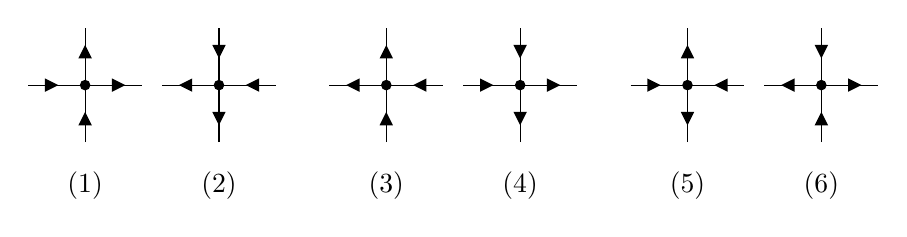
\begin{tikzpicture}
\begin{scope}[scale=0.85]
\VertexRU{0}{0}
\VertexLD{2}{0}
\VertexLU{4.5}{0}
\VertexRD{6.5}{0}
\VertexOne{9}{0}
\VertexMinus{11}{0}
\node at (0,-1.5) {$(1)$};
\node at (2,-1.5) {$(2)$};
\node at (4.5,-1.5) {$(3)$};
\node at (6.5,-1.5) {$(4)$};
\node at (9,-1.5) {$(5)$};
\node at (11,-1.5) {$(6)$};
\end{scope}
\end{tikzpicture}
\caption{\label{fig: 6-vert} The six possible configurations at a vertex.} 
\end{center}
\end{figure}
It is well known that configurations of the six-vertex model with DWBC are mapped bijectively to ASMs by replacing the fifth vertex configurations in Figure~\ref{fig: 6-vert} by a $1$ entry, the sixth configuration by a $-1$ entry and the other configurations by $0$ entries. For an example see Figure~\ref{fig: asm to 6vert}.
\begin{figure}
\begin{center}
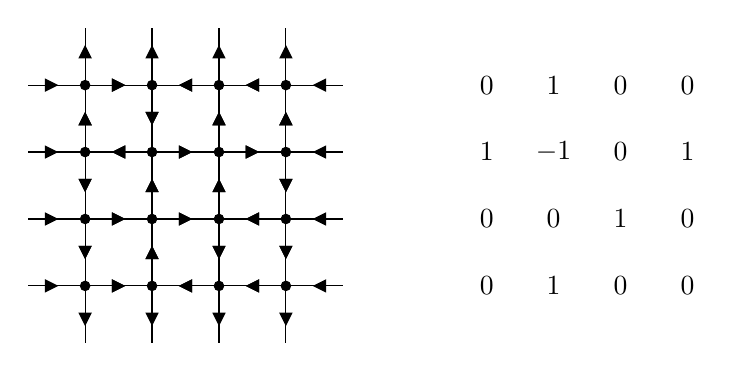
\begin{tikzpicture}
\begin{scope}[scale=0.85]
\VertexRU{0}{0}
\VertexRU{2}{-1}
\VertexRU{1}{-2}
\VertexLU{2}{0}
\VertexLU{3}{0}
\VertexRD{0}{-2}
\VertexRD{0}{-3}
\VertexLD{2}{-3}
\VertexLD{3}{-3}
\VertexLD{3}{-2}
\VertexOne{1}{0}
\VertexOne{0}{-1}
\VertexOne{3}{-1}
\VertexOne{2}{-2}
\VertexOne{1}{-3}
\VertexMinus{1}{-1}
\begin{scope}[xshift=6cm]
\node at (0,0) {$0$};
\node at (1,0) {$1$};
\node at (2,0) {$0$};
\node at (3,0) {$0$};
\node at (0,-1) {$1$};
\node at (1,-1) {$-1$};
\node at (2,-1) {$0$};
\node at (3,-1) {$1$};
\node at (0,-2) {$0$};
\node at (1,-2) {$0$};
\node at (2,-2) {$1$};
\node at (3,-2) {$0$};
\node at (0,-3) {$0$};
\node at (1,-3) {$1$};
\node at (2,-3) {$0$};
\node at (3,-3) {$0$};
\end{scope}
\end{scope}
\end{tikzpicture}
\end{center}
\caption{\label{fig: asm to 6vert} A configuration of the six-vertex model with DWBC and its corresponding ASM.}
\end{figure}
For an ASM $A$, we denote by $\nu_i(A)$ the number of configurations of type $(1)$ and $(2)$ in the $i$-th row of the corresponding six-vertex configuration and by $\mu_i(A)$ the number of configurations of type $(6)$ in row $i$. 
In~\cite{Behrend13}, Behrend considered the following generating function of ASMs
\begin{multline*}
X_n(u,w;x_1,\ldots,x_n)\\
 = Z_n^{1,2,\ldots,n}(u,w;x_1,\ldots,x_n;u x_1^2 + (w-u-1)x_1+1, \ldots, 	u x_n^2 + (w-u-1)x_n+1) \\
= \sum_{A \in \ASM_n} u^{\inv(A)} \prod_{i=1}^n x_i^{\nu_i(A)} (u x_i^2 + (w-u-1)x_i+1)^{\mu_i(A)}. 
\end{multline*}
For the definitions of $X_n$ and $Z_n$, see \cite[Eqs. 67, 70, 73]{Behrend13} and, for the statistics $\nu_i$ and $\mu_i$ compare also to \cite[Eqs. 113, 2]{Behrend13}. In the following, we show that the function $X_n$ satisfies
\begin{equation}
\label{eq: connection to X}
\sum_{A \in \ASM_n}  \omega_A(u,1,w;\x)  = X_n(u,1+u+w;\x).
\end{equation}
For an ASM $A$, let $M=(m_{i,j})$ be the monotone triangle associated to $A$. The equation~\eqref{eq: connection to X} is an easy consequence of the identities $s_{i-1}(M)=\mu_i(A)$ and $\nu_i(A) = \widehat{d}_i(M)-s_{i-1}(M)$. The first identity follows directly from the bijections between monotone triangles, ASMs and configurations of the six-vertex model. In the remainder of this section, we prove the second identity.

Let $a_0,\ldots,a_l$ (resp. $b_1,\ldots,b_l$) be the positions of the $1$ (resp. $-1$) entries in row $i$. By the definition of the bijection between monotone triangles and ASMs, we have
\begin{align*}
\{a_0,\ldots,a_l\} &= \{m_{i,1}, \ldots ,m_{i,i} \} \setminus \{ m_{i-1,1}, \ldots , m_{i-1,i-1}\},\\
\{b_1,\ldots,b_l\} &= \{ m_{i-1,1}, \ldots , m_{i-1,i-1}\} \setminus \{m_{i,1}, \ldots ,m_{i,i} \}.
\end{align*}
Note that the second equality implies $l=s_{i-1}(M)$.
In the corresponding six-vertex configuration, the vertex configurations of type $(1)$ correspond to~$0$ entries in the ASM that satisfy the following two conditions: (a) they are left of the first $1$ or between a $-1$ and the following $1$, and (b) the entries in the same column and above the $0$ sum to $0$. There are $(a_0-1) + \sum_{j=1}^l (a_j-b_j-1)$ entries satisfying condition (a). On the other hand, it is not difficult to see that the $0$ entries which satisfy (a) but not (b) are exactly in the columns corresponding to a left-leaning entry of $M$ in row $i-1$, i.e., there are $l_{i-1}(M)$ such entries. Configurations of type $(2)$ correspond to~$0$ entries between a $1$ and the following $-1$ entry with the property that the entries in the same column and above the $0$ sum to $1$. These positions correspond to the right-leaning entries in $M$ in row $i-1$, hence there are $r_{i-1}(M)$ such entries. Putting this all together, we have
\begin{multline*}
\nu_i(A) = (a_0-1) + \sum_{j=1}^l (a_j-b_j-1)  - l_{i-1}(M) + r_{i-1}(M)\\
= \sum_{j=1}^i m_{i,j} - \sum_{j=1}^{i-1} m_{i-1,j}  -s_{i-1}(M)-1- l_{i-1}(M) + r_{i-1}(M)
=\widehat{d}_i(M)  -s_{i-1}(M).
\end{multline*}

\section{An antisymmetrizer to determinant formula}
\label{sec: antisym to det}
In this section we provide a fundamental tool for the proof of Theorem~\ref{thm: main thm 1}. We present both a non-combinatorial proof next and a combinatorial proof for it in the appendix. The first 
application of the lemma is indeed the proof of the Theorem~\ref{thm: main thm 1}, however 
more applications are given in~\cite{FH2022,FischerSchreierAigner23}.

\begin{lemm}  
\label{lem: general}
Let $n \ge 1$, and $\mathbb{X}=(X_1,\ldots,X_n), \mathbb{Y}=(Y_1,\ldots,Y_n)$ be indeterminants.
 Then
\[
\widehat{\asym}  \left[  \prod_{1 \le i \le j \le n} (Y_j-X_i)     \right]
= \det_{1 \le i, j \le n} \left( Y_i^j - X_i^j \right),
\]
where $\widehat{\asym}$ is the antisymmetrizer with respect to two sets of variables which is defined as
\[
\widehat{\asym} \left[f(\mathbb{X};\mathbb{Y})\right] = \sum_{\sigma \in {\mathcal{S}_n}} \sgn \sigma f(X_{\sigma(1)},\ldots,X_{\sigma(n)};Y_{\sigma(1)},\ldots,Y_{\sigma(n)}).
\] 
\end{lemm}

\begin{proof}
Since we aim that proving the equality of two polynomials in $X_1,\ldots,X_n,\allowbreak Y_1,\ldots,Y_n$, standard arguments imply that it suffices to consider the case when $X_1,\ldots,X_n,\allowbreak Y_1,\ldots,Y_n$ are algebraically independent. In particularly, we may assume $\det_{1 \le i, j \le n} \left( Y_i^j - X_i^j \right) \not=0$, which will be useful below.

The proof is by induction with respect to $n$. The result is obvious for $n=1$. 
Let $L_n(\mathbb{X};\mathbb{Y})$, $R_n(\mathbb{X};\mathbb{Y})$ denote the left- and right-hand side of the identity in the statement, respectively. By the induction hypothesis, we can assume 
that $ L_{n-1}(Y_1,\ldots,Y_{n-1};X_1,\ldots,X_{n-1}) = R_{n-1}(Y_1,\ldots,Y_{n-1};X_1,\ldots,X_{n-1})$.
We show that both $L_n(\mathbb{X};\mathbb{Y})$ and $R_n(\mathbb{X};\mathbb{Y})$ can be computed recursively using 
$L_{n-1}(X_1,\ldots,X_{n-1};Y_1,\ldots,Y_{n-1})$ and $R_{n-1}(X_1,\ldots,X_{n-1};Y_1,\ldots,Y_{n-1})$, respectively, with the same recursion.
For the left-hand side, we have 
\begin{multline}
\label{eq:recursion left}
L_n(\mathbb{X};\mathbb{Y}) \\
=  \sum_{i=1}^{n} (-1)^{i+1}  \left( \prod_{k=1}^n (Y_k-X_i)  \right) 
L_{n-1}(X_1,\ldots,\widehat{X_i},\ldots,X_n;Y_1,\ldots,\widehat{Y_i},\ldots,Y_n),
\end{multline}
where $\widehat{X_i}$ and $\widehat{Y_i}$ means that $X_i$ and $Y_i$ are omitted.
In order to deal with the right-hand side, we first observe
\begin{equation}
\label{fundamentalidentity}
\sum_{j=0}^{n} (Y_i^j - X_i^j) e_{n-j}(-Y_1,\ldots,-Y_n) = (-1)^{n-1} \prod_{k=1}^{n} (Y_k-X_i),
\end{equation}
where $e_{j}(Y_1,\ldots,Y_n)$ denotes the $j$-th elementary symmetric function. Note that the summand for $j=0$ on the left-hand side is actually $0$, and can therefore be omitted.
Now consider the following system of linear equations with $n$ unknowns $c_j(\mathbb{X};\mathbb{Y})$, $1 \le j \le n$.
\[
\sum_{j=1}^{n} (Y_i^j - X_i^j)  c_j(\mathbb{X};\mathbb{Y})
= (-1)^{n-1} \prod_{k=1}^{n} (Y_k-X_i), \quad 1 \le i \le n.
\]
The determinant of this system of equations is obviously $R_n(\mathbb{X};\mathbb{Y})$ and can be assumed to be non-zero. By~\eqref{fundamentalidentity}, we know that the unique solution of this system is given by 
$
c_j(\mathbb{X};\mathbb{Y}) = e_{n-j}(-Y_1,\ldots,-Y_n).
$
On the other hand, by Cramer's rule, 
\[
c_n(\mathbb{X};\mathbb{Y}) = \frac{\det \limits_{1 \le i, j \le n} \left( \begin{cases}  Y_i^j - X_i^j, & \text{if $j<n$} \\
  (-1)^{n-1} \prod\limits_{k=1}^{n} (Y_k-X_i) , & \text{if $j=n$}  \end{cases} \right)}{R_n(\mathbb{X};\mathbb{Y})}.
\]
The assertion now follows from $c_n(\mathbb{X};\mathbb{Y}) = e_{0}(-Y_1,\ldots,-Y_n)=1$, since expanding the determinant in the numerator with respect to the last column yields the recursion~\eqref{eq:recursion left} with $L_{n-1}$ replaced by $R_{n-1}$.
\end{proof}

\section{The Schur expansion of the symmetric generating function}
\label{sec: proof of mt 1}

In order to prove Theorem~\ref{thm: main thm 1}, we first derive an explicit expansion of the symmetric generating function into Schur polynomials. Second, we prove that the coefficients of each Schur polynomial satisfy the same recursion as the right hand side of~\eqref{eq: main thm 1}.
Let $\asym$ denote the antisymmetrizer, i.e.,
\[
\asym_{\x}  f(\mathbf{x}) = \sum\limits_{\sigma \in {\mathcal S}_n} \sgn(\sigma) \allowbreak \cdot f(x_{\sigma(1)},\ldots,x_{\sigma(n)})
.
\] 
We can rewrite the classical bialternant formula for Schur polynomials using the antisymmetrizer and obtain for the operator formula in~\eqref{eq: sym gen fct via Operatoren}
\begin{multline*}
 \left. \left[ \prod_{1 \leq i < j \leq n} \left(u E_{\lambda_i}  + w E_{\lambda_i}E_{\lambda_j}^{-1} +  v E_{\lambda_j}^{-1}  \right) s_{(\lambda_n,\ldots,\lambda_1)}(\x) \right] \right|_{\lambda_i=i-1} \\
=  \left. \left[ \prod_{1 \leq i < j \leq n} \left(u E_{\lambda_i}  + w E_{\lambda_i}E_{\lambda_j}^{-1} +  v E_{\lambda_j}^{-1}  \right) \frac{\asym_\x \left[\prod\limits_{i=1}^n x_i^{\lambda_i+i-1}\right]}{\prod\limits_{1 \leq i < j \leq n}(x_j-x_i)} \right] \right|_{\lambda_i=i-1} \\
=  \left.  \frac{\asym_\x \left[\prod\limits_{1 \leq i < j \leq n} \left(u E_{\lambda_i}  + w E_{\lambda_i}E_{\lambda_j}^{-1} +  v E_{\lambda_j}^{-1}  \right) \cdot \prod\limits_{i=1}^n x_i^{\lambda_i+i-1}\right]}{\prod\limits_{1 \leq i < j \leq n}(x_j-x_i)} \right|_{\lambda_i=i-1}.
\end{multline*}
Since applying $E_{\lambda_i}$ to  $x_i^{\lambda_i}$ has the same effect as multiplication by $x_i$, we obtain further
\begin{equation}  \frac{\asym_\x \left[
\prod\limits_{1 \leq i < j \leq n} \left(u x_i  + w x_i x_j^{-1} +  v x_j^{-1}  \right) \prod\limits_{i=1}^n x_i^{2(i-1)} \right]}{\prod\limits_{1 \leq i < j \leq n}(x_j-x_i)}. \label{eq: sym gen fct via antisym}
\end{equation} 
 By multiplying the $(i,j)$-th factor in the product with $x_i^{-1} x_j$ and multiplying the antisymmetrizer by the symmetric function $\prod_i x_i^{-(n-1)}(v x_i^{-1}+w+ux_i)$,
  we arrive at
\begin{multline*}
\prod\limits_{i=1}^n \left( \frac{ x_i^{n-1}}{\frac{ v}{x_i} + w + u x_i} \right)
   \frac{ \asym_{\x} 
\left[  \prod\limits_{1 \le i \le  j \le n} \left(\frac{ v}{x_i} + w + u x_j\right) \right]}{ \prod\limits_{1 \le i < j \le n} (x_j - x_i)}
=\\
\prod\limits_{i=1}^n \left( \frac{ x_i^{n-1}}{\frac{ v}{x_i} + w + u x_i} \right)
   \frac{ \asym_{\x} 
\left[  \prod\limits_{1 \le i \le  j \le n} \left(\frac{ v}{x_j} + w + u x_i\right) \right]}{ \prod\limits_{1 \le i < j \le n} (x_i - x_j)},
\end{multline*}
where we replaced $x_i$ by $x_{n+1-i}$ for all $i$ in both the numerator and denominator.
We apply Lemma~\ref{lem: general} for $X_i=-w-u x_i$ and $Y_i=v x_i^{-1}$, 
and obtain
\begin{equation}
\label{eq: sym gen fct via det}
\frac{\det_{1 \leq i,j \leq n}\left( x_i^{n-j}p_j(x_i) \right)}{\prod_{1 \leq i < j \leq n}(x_i-x_j)},
\end{equation}
where 
\[
p_j(x) = x^{j-1}\frac{v^j x^{-j}-\left( -w-u x\right)^j}{(v x^{-1}+w+u x)}
= \sum\limits_{k=0}^{j-1}x^k(-w-u x)^k  v^{j-k-1}.
\]
 To emphasise the general principle used to express the determinantal expression in~\eqref{eq: sym gen fct via det} as a sum of Schur polynomials, we consider $q_j(x)$ to be a family of polynomials $q_j(x):= \sum_{k\geq 0} a_{j,k} x^k$.
Using the linearity of the determinant in the columns, we have
\begin{equation}
\label{eq: det to Schur I}
\frac{\det\limits_{1 \leq i,j \leq n}\left( x_i^{n-j}q_j(x_i) \right)}{\prod\limits_{1 \leq i< j \leq n}(x_i-x_j)}
= \sum\limits_{k_1,\ldots,k_n \geq 0} \left( \prod_{j=1}^n a_{j,k_j} \right) s_{(k_1,\ldots, k_n)}(\mathbf{x}),
\end{equation}
where we used the well known extension of Schur polynomials to arbitrary sequences $L=(L_1,\ldots,L_n)$ of non-negative integers via
\[
s_{L}(\mathbf{x}) := \frac{\det\limits_{1 \leq i,j \leq n}\left( x_i^{L_j+n-j}\right)}{\prod\limits_{1 \leq i < j \leq n}(x_i-x_j)}.
\]
It can be checked that the generalised Schur polynomial $s_L(\mathbf{x})$ is either equal to~$0$ or $s_L(\mathbf{x})= \sgn(\sigma) s_\lambda(\mathbf{x})$ where $\lambda=(\lambda_1,\ldots, \lambda_n)$ is a partition 
and $\sigma \in S_n$ is a permutation such that $L_j=\lambda_{\sigma(j)}+j-\sigma(j)$ for all $1 \leq j \leq n$. It follows that~\eqref{eq: det to Schur I} is equal to
\begin{equation}
\label{eq: det to Schur II}
 \sum_{\lambda} s_\lambda(\mathbf{x}) \left( \sum_{\sigma \in S_n} \sgn(\sigma) \prod_{j=1}^n a_{j,\lambda_{\sigma(j)}+j-\sigma(j)}  \right)
= \sum_{\lambda} s_\lambda(\mathbf{x}) \det\limits_{1 \leq i,j \leq n} \left( a_{j,\lambda_i+j-i} \right),
\end{equation}
where the sum is over all partitions $\lambda$.
By applying~\eqref{eq: det to Schur II} to the family of polynomials 
\[
p_{j}(x) 
=\sum\limits_{k=0}^{j-1}x^k(-w-u x)^k  v^{j-k-1}
= \sum\limits_{k=0}^{j-1} \sum\limits_{l\geq 0}
(-1)^{k}\binom{k}{l} x^{k+l}   u^lv^{j-k-1} w^{k-l}
,
\]
we obtain
\begin{multline*}
\sum_{A \in \ASM_n}\omega_A(u,v,w;\x) \\=
\sum_\lambda s_\lambda(\mathbf{x}) \det\limits_{1 \leq i,j \leq n} \left( 
\sum\limits_{k=0}^{j-1}  \sum\limits_{\substack{l \geq 0 \\ k+l = \lambda_i+j-i}}
(-1)^{k}\binom{k}{l}   u^lv^{j-k-1} w^{k-l}
\right)\\
= \sum_\lambda s_\lambda(\mathbf{x})  \det_{1 \leq i,j \leq n} \left(
\sum_{k=0}^{j-1} (-1)^{k}\binom{k}{\lambda_i+j-i-k} u^{\lambda_i+j-i-k} v^{j-k-1} w^{2k+i-\lambda_i-j}
\right).
\end{multline*}

We denote by $m_{i,j}(\lambda_i)$ the $(i,j)$-th entry of the matrix in the above determinant. An entry $m_{i,1}(\lambda_i)= \binom{0}{\lambda_i+1-i}u^{\lambda_i+1-i} w^{i-\lambda_i-1} $ in the first column is $1$ iff $\lambda_i=i-1$ and $0$ otherwise. Let $l$ be the side length of the Durfee square of $\lambda$. The only possible part of $\lambda$ satisfying $\lambda_i=i-1$ is the $(l+1)$-st. Hence we assume for the rest of the proof $\lambda_{l+1}=l$. By expanding the determinant along the first column, we obtain
\[
\det_{1 \leq i,j \leq n} \left(m_{i,j}(\lambda_i) \right) = (-1)^{l+2}\det_{1 \leq i,j \leq n-1} \left(m_{i,j}^\prime \right),
\]
where $(m_{i,j}^\prime)_{1,\leq,i,j \leq n-1}$ denotes the matrix obtained by deleting the first column and the $(l+1)$-st row of $(m_{i,j}(\lambda_i))_{1\leq i,j \leq n}$. For $1 \leq i \leq l$, in which case we have $\lambda_{i}\geq i$, we can rewrite $m_{i,j}^\prime$ as
\begin{multline*}
m_{i,j}^\prime =
\sum_{k=0}^{j} (-1)^k \binom{k}{\lambda_i+(j+1)-i-k}  u^{\lambda_i+(j+1)-i-k} v^{(j+1)-k-1} w^{2k+i-\lambda_i-(j+1)} \\
= \sum_{k=0}^{j-1} (-1)^{k+1}    u^{\lambda_i+j-i-k}v^{j-k-1} w^{2k+1+i-\lambda_i-j} \\
\times
 \left( \binom{k}{\lambda_i+j-i-k}+ \binom{k}{\lambda_i+j-i-k-1} \right) \\
 = -w \, m_{i,j}(\lambda_i) - u \, m_{i,j}(\lambda_i-1).
\end{multline*}
For $i>l$ on the other hand, i.e., $\lambda_{i+1}<i$, we can express $m_{i,j}^\prime$ analogously as
\begin{multline*}
m_{i,j}^\prime = \sum_{k=0}^{j} (-1)^{k}\binom{k}{\lambda_{i+1}+(j+1)-(i+1)-k} \\
\times  u^{\lambda_{i+1}+(j+1)-(i+1)-k} v^{(j+1)-k-1} w^{2k+(i+1)-\lambda_{i+1}-(j+1)}
=  v m_{i,j}(\lambda_{i+1}),
\end{multline*}
where the sum has been extended, which is allowed since $\binom{j}{\lambda_{i+1}-i}=0$.
Summarising, we denote by $c_{n,\lambda}$ the coefficient of $s_\lambda(\mathbf{x})$ in the symmetric generating function $\sum_{A \in \ASM_n}\omega_A(u,v,w;\x)$. Then
\begin{multline*}
c_{n,\lambda} =\\
 (-1)^{l}\det_{1 \leq i,j \leq n-1} \left(m_{i,j}^\prime \right) 
 = (-1)^{l}\det_{1 \leq i,j \leq n-1} \left( 
\begin{cases}
-w m_{i,j}(\lambda_i)- u m_{i,j}(\lambda_i-1), \quad & i \leq l\\
 v m_{i,j}(\lambda_{i+1}), & i>l
\end{cases} \right) \\
= \sum_{(f_1,\ldots,f_l) \in \{0,1\}^l} u^{\sum_{i=1}^l f_i}  v^{n-1-l} w^{l-\sum_{i=1}^l f_i}
  c_{n-1,(\lambda_1 -f_1,\ldots,\lambda_l-f_l,\lambda_{l+2},\ldots,\lambda_n)},
\end{multline*}
with $c_{n-1,(\lambda_1 -f_1,\ldots,\lambda_l-f_l,\lambda_{l+2},\ldots,\lambda_n)}=0$ if $(\lambda_1 -f_1,\ldots,\lambda_l-f_l,\lambda_{l+2},\ldots,\lambda_n)$ is not a partition, where the equality follows from the linearity of the determinant in the rows and choosing $f_i=0$ iff we select the first term in row $i$.
Using Frobenius notation for $\lambda=(a_1,\ldots,a_l|b_1,\ldots,b_l)$, the above recursion can be rewritten as
\begin{multline*}
c_{n,(a_1,\ldots,a_l|b_1,\ldots,b_l)} \\
= \sum_{(f_1,\ldots,f_l) \in \{0,1\}^l} u ^{\sum_{i=1}^l f_i} v^{n-1-l} w^{l-\sum_{i=1}^l f_i}  c_{n-1,(a_1-f_1,\ldots,a_l-f_l|b_1-1,\ldots,b_l-1)},
\end{multline*}
where $c_{n-1,(a_1,\ldots,a_{l-1},-1|b_1,\ldots,b_{l-1},0)}$ is defined as $c_{n-1,(a_1,\ldots,a_{l-1}|b_1,\ldots,b_{l-1})}$ .

Denote by $d_{n,\lambda}$ the coefficient of $s_\lambda(\x)$ in $\A_{n,1}(1, u,v,w;\x)$. For $\lambda=(a_1,\ldots,a_l| \allowbreak b_1,\ldots,b_l)$, Proposition~\ref{prop: TSSPP refinement} implies 
\begin{multline*}
d_{n,(a_1,\ldots,a_l|b_1,\ldots,b_l)} 
= u^{\sum_{i=1}^l (a_i+1)} v^{\binom{n}{2}-\sum_{i=1}^l b_i} w^{\sum_{i=1}^l(b_i-1-a_i)} 
 \det_{1 \leq i,j \leq l} \left( \binom{b_j-1}{a_i} \right)\\
= u^{\sum_{i=1}^l (a_i+1)} v^{\binom{n}{2}-\sum_{i=1}^l b_i} w^{\sum_{i=1}^l(b_i-1-a_i)} 
 \det_{1 \leq i,j \leq l} \left( \binom{b_j-2}{a_i}+\binom{b_j-2}{a_i-1} \right)\\
 =  \sum_{(f_1,\ldots,f_l) \in \{0,1\}^l}  u^{\sum_{i=1}^l f_i} v^{n-1-l} w^{l-\sum_{i=1}^l f_i} 
 d_{n-1,(a_1-f_1,\ldots,a_l-f_l|b_1-1,\ldots,b_l-1)},
\end{multline*}
where we used the linearity of the determinant in the last step. The assertion follows by induction on $n$ since both $c_{n,\lambda}$ and $d_{n,\lambda}$ satisfy the same recursion and the induction base can be checked easily. This proves Theorem~\ref{thm: main thm 1}.

\begin{thebibliography}{MMMMMM}
\bibitem[1]{Aigner21} Aigner, Florian A new determinant for the Q-enumeration of alternating sign matrices, J. Combin. Theory Ser. A, Volume 180 (2021), Paper no. 105412, 27 pages \href{https://alco.centre-mersenne.org/articles/10.5802/alco.374/#Aigner21}{Publisher reference}.
\bibitem[2]{AignerFischerKonvalinkaNadeauTewari20} Aigner, Florian; Fischer, Ilse; Konvalinka, Matjaž; Nadeau, Philippe; Tewari, Vasu Alternating sign matrices and totally symmetric plane partitions, Sém. Lothar. Combin., Volume 84B (2020), Paper no. 77, 12 pages \href{https://alco.centre-mersenne.org/articles/10.5802/alco.374/#AignerFischerKonvalinkaNadeauTewari20}{Publisher reference}.
\bibitem[3]{Andrews79} Andrews, George E. Plane partitions. III. The weak Macdonald conjecture, Invent. Math., Volume 53 (1979) no. 3, pp. 193-225 \href{https://alco.centre-mersenne.org/articles/10.5802/alco.374/#Andrews79}{Publisher reference}.
\bibitem[4]{Andrews94} Andrews, George E. Plane partitions. V. The TSSCPP conjecture, J. Combin. Theory Ser. A, Volume 66 (1994) no. 1, pp. 28-39 \href{https://alco.centre-mersenne.org/articles/10.5802/alco.374/#Andrews94}{Publisher reference}.
\bibitem[5]{Bailey35} Bailey, W. N. Generalized hypergeometric series, Cambridge Tracts in Mathematics and Mathematical Physics, No. 32, Stechert-Hafner, Inc., New York, 1964, v+108 pages \href{https://alco.centre-mersenne.org/articles/10.5802/alco.374/#Bailey35}{Publisher reference}.
\bibitem[6]{Behrend13} Behrend, Roger E. Multiply-refined enumeration of alternating sign matrices, Adv. Math., Volume 245 (2013), pp. 439-499 \href{https://alco.centre-mersenne.org/articles/10.5802/alco.374/#Behrend13}{Publisher reference}.
\bibitem[7]{Fischer05} Fischer, Ilse A method for proving polynomial enumeration formulas, J. Combin. Theory Ser. A, Volume 111 (2005) no. 1, pp. 37-58 \href{https://alco.centre-mersenne.org/articles/10.5802/alco.374/#Fischer05}{Publisher reference}.
\bibitem[8]{Fischer06} Fischer, Ilse The number of monotone triangles with prescribed bottom row, Adv. in Appl. Math., Volume 37 (2006) no. 2, pp. 249-267 \href{https://alco.centre-mersenne.org/articles/10.5802/alco.374/#Fischer06}{Publisher reference}.
\bibitem[9]{Fischer18} Fischer, Ilse Constant term formulas for refined enumerations of Gog and Magog trapezoids, J. Combin. Theory Ser. A, Volume 158 (2018), pp. 560-604 \href{https://alco.centre-mersenne.org/articles/10.5802/alco.374/#Fischer18}{Publisher reference}.
\bibitem[10]{FH2022} Fischer, Ilse; Höngesberg, Hans Alternating sign matrices with reflective symmetry and plane partitions: n+3 pairs of equivalent statistics, 2022 \href{https://alco.centre-mersenne.org/articles/10.5802/alco.374/#FH2022}{Publisher reference}.
\bibitem[11]{cube} Fischer, Ilse; Konvalinka, Matjaž The mysterious story of square ice, piles of cubes, and bijections, Proc. Natl. Acad. Sci. USA, Volume 117 (2020) no. 38, pp. 23460-23466 \href{https://alco.centre-mersenne.org/articles/10.5802/alco.374/#cube}{Publisher reference}.
\bibitem[12]{FischerKonvalinka20plus} Fischer, Ilse; Konvalinka, Matjaž A bijective proof of the ASM theorem Part II: ASM enumeration and ASM-DPP relation, Int. Math. Res. Not. IMRN (2022) no. 10, pp. 7203-7230 \href{https://alco.centre-mersenne.org/articles/10.5802/alco.374/#FischerKonvalinka20plus}{Publisher reference}.
\bibitem[13]{FischerSchreierAigner23} Fischer, Ilse; Schreier-Aigner, Florian The relation between alternating sign matrices and descending plane partitions: n+3 pairs of equivalent statistics, Adv. Math., Volume 413 (2023), Paper no. 108831, 47 pages \href{https://alco.centre-mersenne.org/articles/10.5802/alco.374/#FischerSchreierAigner23}{Publisher reference}.
\bibitem[14]{GasperRahman90} Gasper, George; Rahman, Mizan Basic hypergeometric series, Encyclopedia of Mathematics and its Applications, 35, Cambridge University Press, Cambridge, 1990, xx+287 pages \href{https://alco.centre-mersenne.org/articles/10.5802/alco.374/#GasperRahman90}{Publisher reference}.
\bibitem[15]{GesselViennot85} Gessel, Ira; Viennot, Gérard Binomial determinants, paths, and hook length formulae, Adv. in Math., Volume 58 (1985) no. 3, pp. 300-321 \href{https://alco.centre-mersenne.org/articles/10.5802/alco.374/#GesselViennot85}{Publisher reference}.
\bibitem[16]{Lindstroem73} Lindström, Bernt On the vector representations of induced matroids, Bull. London Math. Soc., Volume 5 (1973), pp. 85-90 \href{https://alco.centre-mersenne.org/articles/10.5802/alco.374/#Lindstroem73}{Publisher reference}.
\bibitem[17]{MacMahon97} MacMahon, P. A. Memoir on the theory of the partition of numbers, I, Lond. Phil. Trans. (A), Volume 187 (1897), pp. 619-673 \href{https://alco.centre-mersenne.org/articles/10.5802/alco.374/#MacMahon97}{Publisher reference}.
\bibitem[18]{MillsRobbinsRumsey82} Mills, W. H.; Robbins, David P.; Rumsey, Howard Jr. Proof of the Macdonald conjecture, Invent. Math., Volume 66 (1982) no. 1, pp. 73-87 \href{https://alco.centre-mersenne.org/articles/10.5802/alco.374/#MillsRobbinsRumsey82}{Publisher reference}.
\bibitem[19]{MillsRobbinsRumsey86} Mills, W. H.; Robbins, David P.; Rumsey, Howard Jr. Self-complementary totally symmetric plane partitions, J. Combin. Theory Ser. A, Volume 42 (1986) no. 2, pp. 277-292 \href{https://alco.centre-mersenne.org/articles/10.5802/alco.374/#MillsRobbinsRumsey86}{Publisher reference}.
\bibitem[20]{RobbinsRumsey86} Robbins, David P.; Rumsey, Howard Jr. Determinants and alternating sign matrices, Adv. in Math., Volume 62 (1986) no. 2, pp. 169-184 \href{https://alco.centre-mersenne.org/articles/10.5802/alco.374/#RobbinsRumsey86}{Publisher reference}.
\bibitem[21]{Stanley99} Stanley, Richard P. Enumerative combinatorics. Vol. 2, Cambridge Studies in Advanced Mathematics, 62, Cambridge University Press, Cambridge, 1999, xii+581 pages \href{https://alco.centre-mersenne.org/articles/10.5802/alco.374/#Stanley99}{Publisher reference}.
\bibitem[22]{Stembridge95} Stembridge, John R. The enumeration of totally symmetric plane partitions, Adv. Math., Volume 111 (1995) no. 2, pp. 227-243 \href{https://alco.centre-mersenne.org/articles/10.5802/alco.374/#Stembridge95}{Publisher reference}.
\bibitem[23]{Striker11} Striker, Jessica A unifying poset perspective on alternating sign matrices, plane partitions, Catalan objects, tournaments, and tableaux, Adv. in Appl. Math., Volume 46 (2011) no. 1-4, pp. 583-609 \href{https://alco.centre-mersenne.org/articles/10.5802/alco.374/#Striker11}{Publisher reference}.
\bibitem[24]{Zeilberger96} Zeilberger, Doron Proof of the alternating sign matrix conjecture, Electron. J. Combin., Volume 3 (1996) no. 2, Paper no. 13, 84 pages \href{https://alco.centre-mersenne.org/articles/10.5802/alco.374/#Zeilberger96}{Publisher reference}.
\end{thebibliography}
\end{document}
